\documentclass{article}
\usepackage[paperwidth=210mm,paperheight=297mm, top = 30mm, bottom = 30mm]{geometry}
%\usepackage[hangul]{kotex}
\usepackage{kotex}
\usepackage[utf8]{inputenc}
\usepackage{enumitem}
\usepackage{indentfirst}
\usepackage{graphicx, subcaption, tikz}
\usepackage{amsmath, amssymb, amsthm, amsfonts, bm}

\title{2020 Spring MAS365 Numerical Analysis HW6}
\author{20160650 채지석}
\date{\today}

\setlist{  
  listparindent=\parindent,
  %parsep=0pt,
}

\newtheorem{prob}{Problem}

\newcommand{\set}[1]{\left\{ {#1} \right\}}
\newcommand{\vecx}{\boldsymbol{x}}
\newcommand{\mat}[1]{\boldsymbol{#1}}
\newcommand{\mata}{\boldsymbol{A}}
\newcommand{\matb}{\boldsymbol{B}}
\newcommand{\rr}{\mathbb{R}}
\newcommand{\nn}{\mathbb{N}}
\newcommand{\zz}{\mathbb{Z}}
\newcommand{\cc}{\mathbb{C}}
\newcommand{\qq}{\mathbb{Q}}
\newcommand{\norm}[1]{\left\lVert#1\right\rVert}
\newcommand{\card}[1]{\left\lvert#1\right\rvert}
\newcommand{\posdef}{\succ\mat{0}}
\newcommand{\psd}{\succeq\mat{0}}
\newcommand{\trace}{\text{trace}}
\newcommand{\comment}[1]{}
\newcommand{\problem}{\begin{prob}\end{prob}}
                    

\begin{document}

\section*{Computer Assignment}
The program which does the required is submitted via KLMS along with this document. Given the two endpoints of the interval \texttt{a} and \texttt{b}, the step size \texttt{h}, and a function \texttt{f}, the program computes the trigonometric interpolating polynomial by first computing the coefficients $\texttt{beta} = [\beta_k]$ of the phase polynomial using the function \texttt{fft} provided by \textsf{numpy} package, and then computing the coefficients $\texttt{A} = [A_j]$, $\texttt{B} = [B_j]$ using the relations between $\beta_k$ and $A_j, B_j$. The computed interpolating polynomials are printed out, as the following figure. 
\begin{center}
    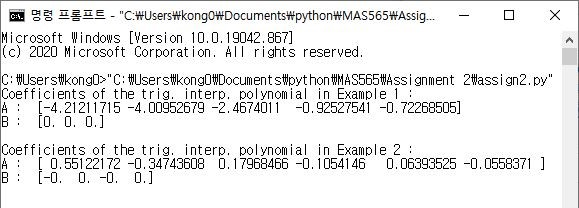
\includegraphics[width=0.8\linewidth]{console.JPG}
\end{center}
As indicated above, the result say that for example the trigonometric interpolating polynomial for the first function as coefficients 
\[
\begin{array}{lllll}
  A_0 = -4.2121, & A_1 = -4.0095, & A_2 = 2.4674, & A_3 = -0.92528, &  A_4 = -0.72269, \\
  & B_1 = 0, & B_2 = 0, & B_3 = 0. &
\end{array}  
\]
The original function $f$ and the interpolating polynomial $p$ plotted together, for the two functions given, is shown as in the following figure. 
\begin{center}
    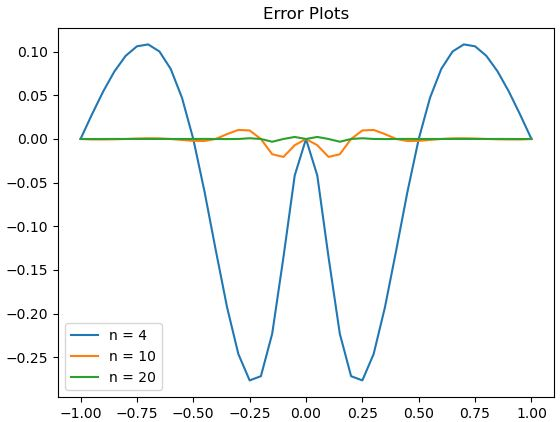
\includegraphics[width=0.85\linewidth]{3313.JPG}
\end{center} \par 
Since both functions given are even functions, we expect that $B_j =0$ for all $j$, and indeed that is the case as we can see in the console output. \par 
For the first function the trigonometric interpolating polynomial is nice, but not great. Our guess is that the nature of $f$, having an M-shaped graph with a very shallow valley, is not well captured with only a few cosine functions. However increasing the number of points in the abscissa shows an improvement in the quality of interpolation. \par 
What is really interesting is the wellness of trigonometric interpolating polynomial interpolating the Runge function. Ordinary polynomials show terrible performance when interpolating the Runge function. But in contrast trigonometric interpolating polynomials well interpolate even the Runge function. Thus, we observe that trigonometric interpolating polynomials have some advantages that ordinary interpolating polynomials do not possess. 

\end{document}